\section{Early Evolution}

Motivated by the popularity of the graphics pipepline, graphics accelerators
in the 1980s and 1990s largely implemented a fixed pipeline in hardware (\cite{mcclanahan2010history}). This section
traces the evolution of this fixed design into one that supports general computation.
This section focuses primarily on Nvidia and their role during this time.

\subsection{Graphics Processing Unit}

With the design of graphics accelerators heavily coupled to the pipeline,
one critical difference between accelerators was how much of the
graphics pipeline did the accelerator actually support.

Until 1999, graphics accelerators did not support the acceleration of
\textit{Transformation} and \textit{Lighting} sub-stages (of the
\textit{Geometry stage}) of the pipeline.
This meant that the CPU would do the \textit{Application} stage and the
the \textit{Transformation} and \textit{Lighting} sub-stages before passing
the resulting vertices to the accelerator to do the rest (\cite{mcclanahan2010history}).

Nvidia was the first company to put the entire \textit{Geometry} stage
onto the accelerator, allowing the CPU to focus on the \textit{Application}
stage \cite{nvidia256}. This meant more high fidelity simulation.

Nvidia marketed this as a graphics processing unit, popularizing the term.

\subsection{Programmability with Shaders}

Processors started to support programmability through what were called shaders.
In hardware, shader units supported code that could be written by the programmer
to specify desired fuctionality at given parts of the pipeline (\cite{mcclanahan2010history}).

Vertex shaders replaced the \textit{Transformation} and \textit{Lighting} parts
of the graphics pipeline. The programmer could specify the specific 
transformations and lighting operations that they wanted performed, as well
as other operations (\cite{lsu}). 

Fragment shaders were added after the \textit{Rasterization} stage.
These enabled the programmer to perform transformations on the fragments
before they were rendered to the screen (\cite{lsu}).

Together, these shaders enabled more advanced graphical features to
be implemented.

\begin{figure}[h]
    \centering
    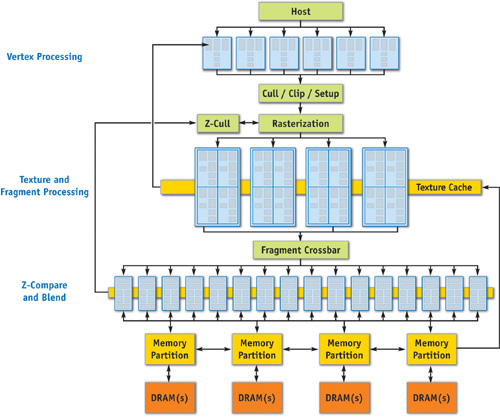
\includegraphics[width=0.75\textwidth]{assets/30_geforce6_03.jpg}
    \caption{Diagram of the GeForce 6 }
    \label{fig:geforce6}
\end{figure}

An example architecture that implemented shaders is in Figure \ref{fig:geforce6} \cite{nvidiaChapterGeForce}.
Note the Vertex Processing (vertex shaders) and Texture and Fragment Processing
(fragment shaders) using different processing units.

\subsection{Unified Shader Architecture}

The unified architecture replaced bespoke hardware for different shaders with
a single processor capable of doing all relevant shader tasks.
This meant that computations for all of these different tasks could be performed
using the same ISA. This ISA thus had to be general, paving the way for
the use of the GPU for applications beyond graphics \cite{parojModernUnification}.

Figure \ref{fig:geforce8} shows Nvidia's GeForce 8 architecture \cite{mcclanahan2010history}. This architecture
has a number of streaming multiprocessors (SMs) with individual streaming processor cores
(SPs). A controller manages what shaders execute on these SMs, allowing their output
to feed back into them.

\begin{figure}[h]
    \centering
    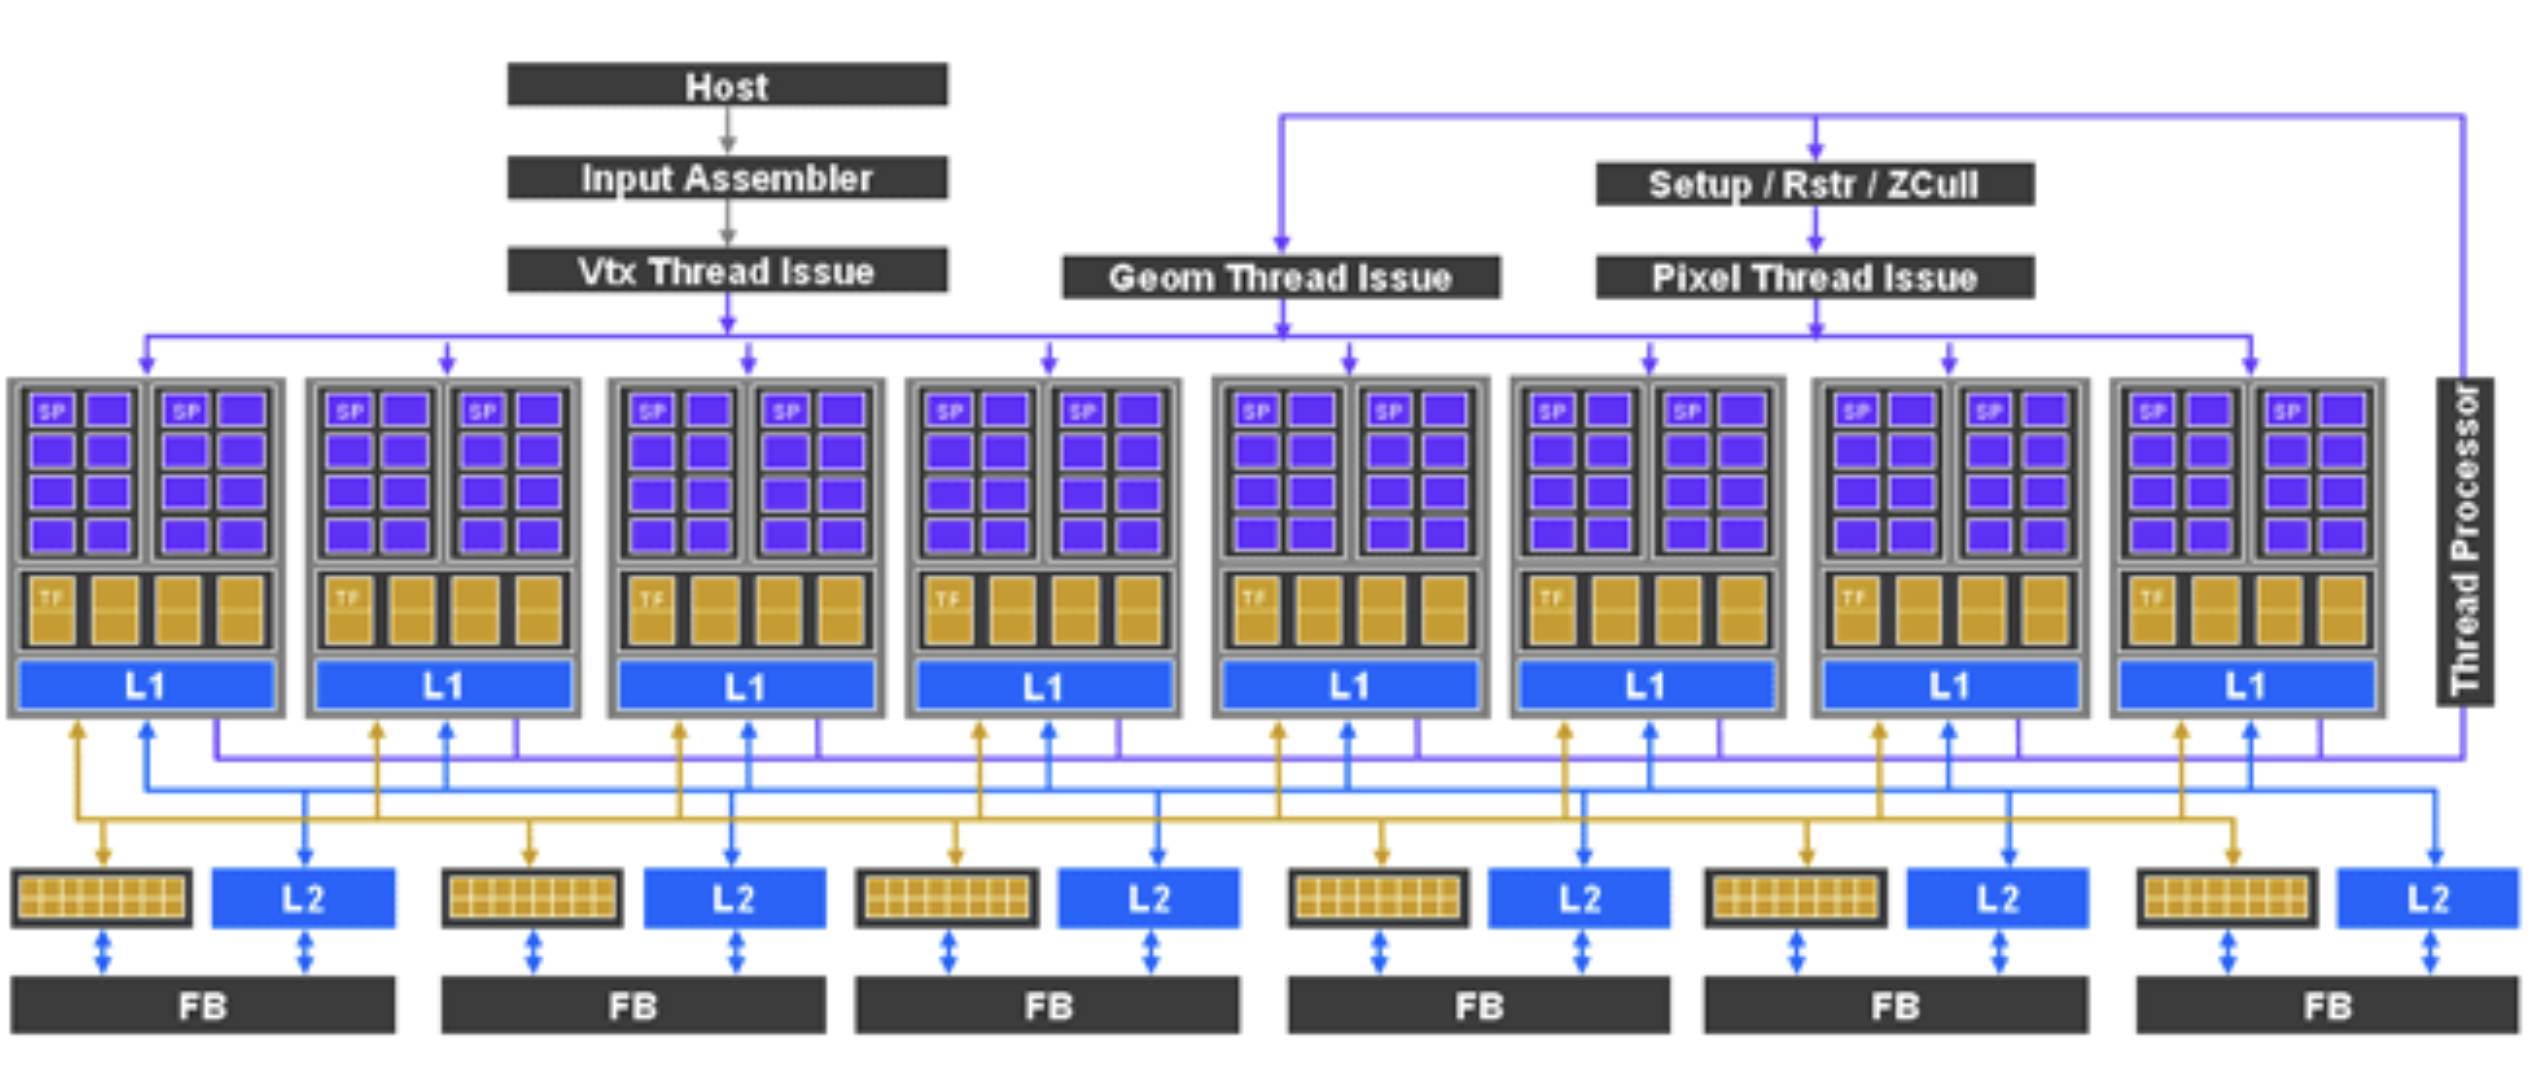
\includegraphics[width=0.75\textwidth]{assets/geforce8.png}
    \caption{Diagram of the GeForce 8.}
    \label{fig:geforce8}
\end{figure}

\subsection{The General Purpose GPU}


\begin{figure}[h]
    \centering
    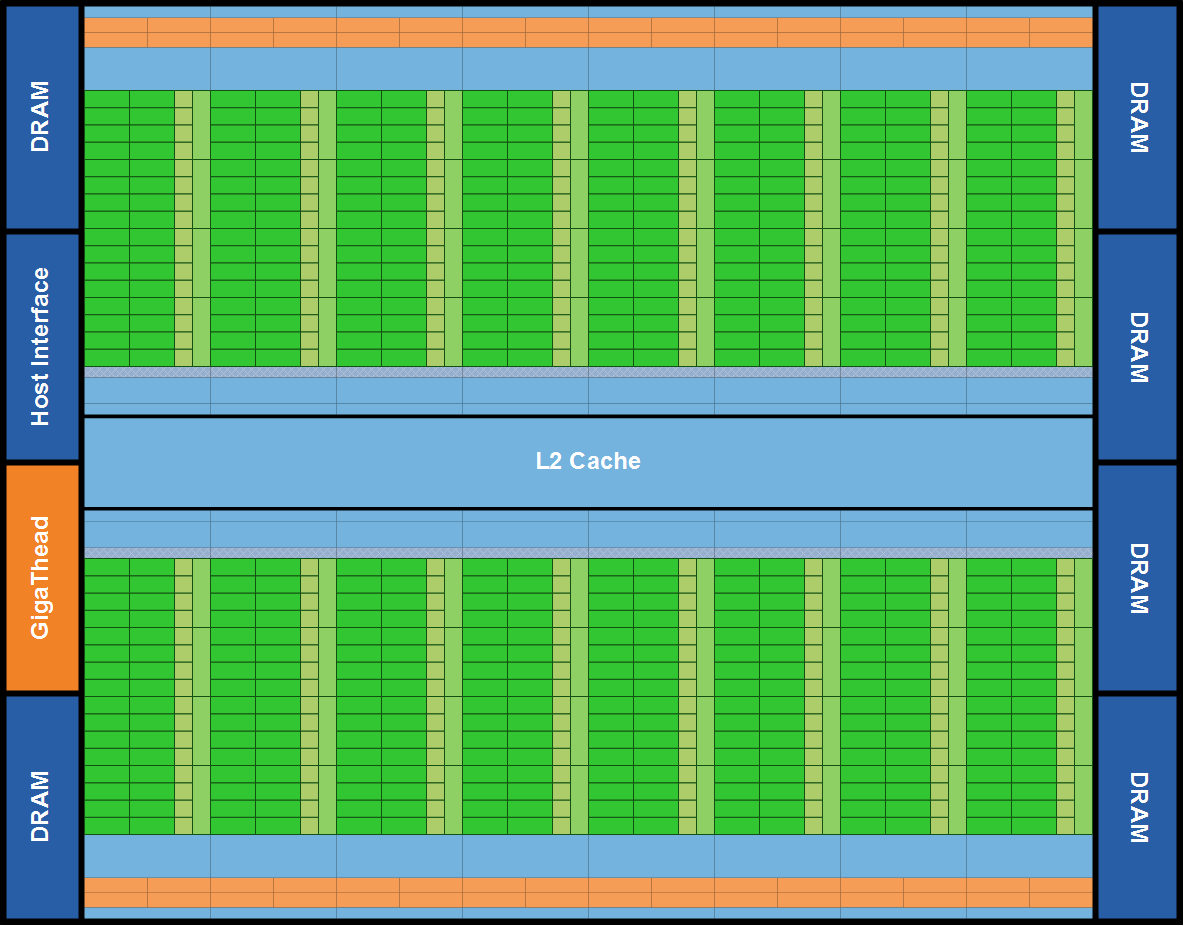
\includegraphics[width=0.5\textwidth]{assets/fermi_architecture1.png}
    \caption{Diagram of the entire Fermi architecture.}
    \label{fig:fermi}
\end{figure}

Nvidia had an interest in general purpose GPU computing at least as early as during the development
of the GeForce 8 series (\cite{dally2021evolution}).
Fermi represented their first card marketed as a general purpose accelerator (\cite{nvidiafermi}).
The general architecture of the chip can be seen in Figure \ref{fig:fermi} and a single 
multiprocessor core can be seen in Figure \ref{fig:fermiSM} (\cite{nvidiafermi}).


\begin{figure}[h]
    \centering
    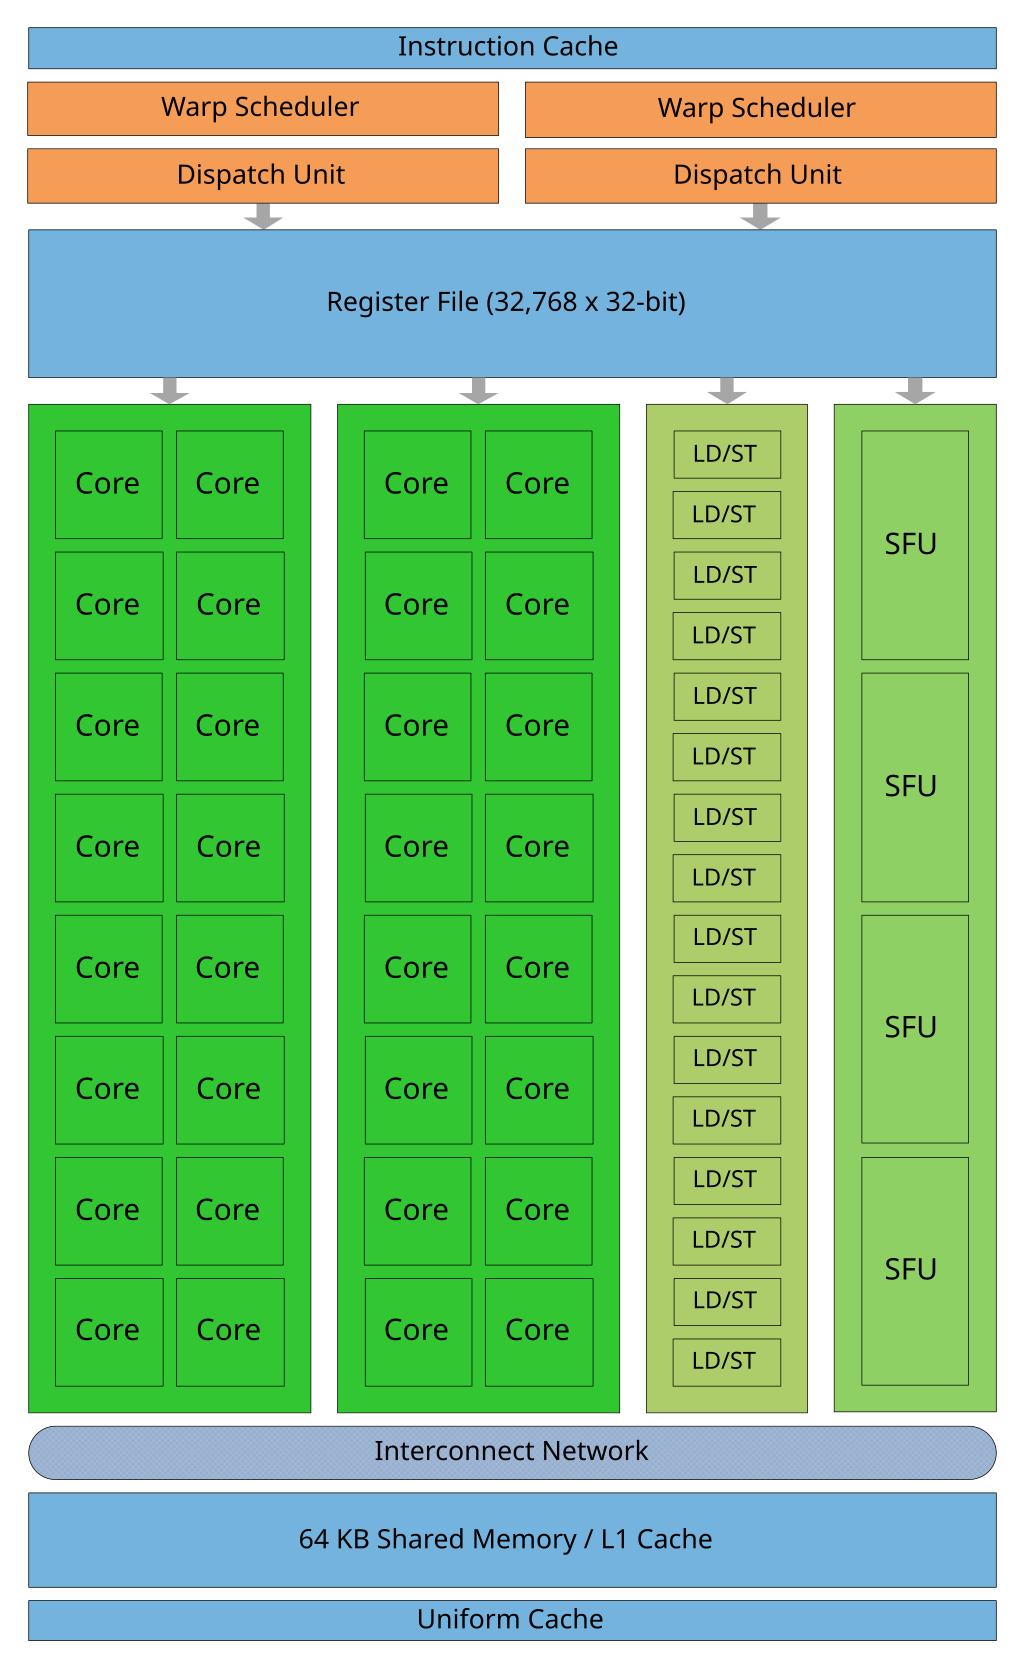
\includegraphics[width=0.5\textwidth]{assets/Fermi.svg.png}
    \caption{Diagram of a single Fermi SM} 
    \label{fig:fermiSM}
\end{figure}
